\documentclass{article}
% \usepackage[a4paper, total={6in, 8in}]{geometry}
\usepackage{xcolor}
\usepackage[detect-all, abbreviations]{siunitx}
\usepackage{physics}
\usepackage{graphicx}
\usepackage[font=small,labelfont=bf]{caption}
\usepackage[subrefformat=parens]{subcaption}
\usepackage{bm}
\usepackage{bbold}
\usepackage[colorlinks=true,linkcolor=blue,urlcolor=blue,citecolor=blue]{hyperref}% add hypertext capabilities
\usepackage[mathlines]{lineno}% Enable numbering of text and display math
% \linenumbers\relax % Commence numbering lines

\title{Two atoms with hyperfine states}
% \author{Kyungtae  Kim}
\date{\today}

\begin{document}
\maketitle

\section{Introduction}
We want to explore the effect of hyperfine states (Fig.~\ref{fig:level_diagram}) on the decay rate of the two atoms. Codes associated with calculations are in the \href{https://github.com/kimkyngt/DecayDynamics}{repository}. We want to address the questions below.
\begin{itemize}
    \item How to properly describe the hyperfine states?
    \item Can coherence between different Zeeman sublevel be transfered through the decay?
    \item How much reduction of the collective effect we can expect by having many branches?
    \item How different is the functional form of the radation power at the detector and the functional form of $^3P_1$ population?
\end{itemize}

\begin{figure}[h]
    \centering
    \includegraphics[width=0.8\textwidth]{level_diagram.pdf}
    \caption{Relavant energy levels of $^{87}$Sr atom. Nuclear spin is 9/2. One of the initial population sheme is presented with red blobs. The bigger the blob, the more population.  \label{fig:level_diagram}}
\end{figure}
\section{Definitions}

We consider magnetic sublevel contributions similar to equation (2) in the reference \cite{asenjo-garciaOpticalWaveguidingAtomic2019}. However, this expression seems to make total decay rate to be dependant on the angular momentum quantum number of the excited state. See \texttt{src/Gamma\_0\_test.jl} to see its dependence. To make total decay rate of a certain level to be $F$-independent, we add a factor $\sqrt{2F_e + 1}$ to the definition of the atomic rasing operator(equation (2) in \cite{asenjo-garciaOpticalWaveguidingAtomic2019}).
$$\begin{gathered}
\hat{\Sigma}_q = \sum_{m_g = -F_g}^{F_g}  \sqrt{2F_e + 1} (-1)^{F_g-m_g}\left(\begin{array}{llc}
F_g & 1 & F_e \\
-m_g & q & m_g-q
\end{array}\right) |F_e m_g-q\rangle \langle F_g m_g |  \\
= \sum_{m_g = -F_g}^{F_g} (-1)^{2m_g - q} |F_g m_g \rangle \langle F_g, m_g; 1, -q| F_e, m_g - q \rangle \langle F_e m_g - q |
\end{gathered}$$
The other parts are essentially the same as \cite{asenjo-garciaOpticalWaveguidingAtomic2019}. As we are considering the cascaded system, we need to consider different transitions. The index $l$ denotes a specific transition; 1 is for $^3D_1 \rightarrow {}^3P_1$, 2 is for $^3D_1 \rightarrow {}^3P_0$, and 3 is for $^3P_1 \rightarrow {}^1S_0$.
$$\begin{gathered}
\mathcal{H} = \hbar \sum_{l=1}^{3}\sum_{i, j=1}^N \sum_{q, q^{\prime}=-1}^1 J_{i j q q^{\prime}}^{(l)} \hat{\Sigma}_{i q}^{(l)\dagger} \hat{\Sigma}_{j q^{\prime}}^{(l)}, \\ 
\mathcal{L}[\rho] = \sum_{l=1}^{3}\sum_{i, j=1}^N \sum_{q, q^{\prime}=-1}^1 \frac{\Gamma_{i j q q^{\prime}}^{(l)}}{2}\left(2 \hat{\Sigma}_{j q^{\prime}}^{(l)} \rho \hat{\Sigma}_{i q}^{(l)\dagger}-\hat{\Sigma}_{i q}^{(l)\dagger} \hat{\Sigma}_{j q^{\prime}}^{(l)} \rho -\rho \hat{\Sigma}_{i q}^{(l)\dagger} \hat{\Sigma}_{j q^{\prime}}^{(l)}\right)
\end{gathered}$$

$$
\begin{aligned}
& J_{i j q q^{\prime}}^{(l)} = -\frac{3}{4}\Gamma^{(l)} \hat{\mathbf{e}}_q \cdot \operatorname{Re} \mathbf{G}\left(\mathbf{r}_i, \mathbf{r}_j, \omega_l\right) \cdot \hat{\mathbf{e}}_{q^{\prime}}^* \\
& \Gamma_{i j q q^{\prime}}^{(l)} = \frac{3}{2}\Gamma^{(l)}  \hat{\mathbf{e}}_q \cdot \operatorname{Im} \mathbf{G}\left(\mathbf{r}_i, \mathbf{r}_j, \omega_l\right) \cdot \hat{\mathbf{e}}_{q^{\prime}}^*
\end{aligned}
$$

$$
\mathbf{G}\left(\mathbf{r}, \omega_l\right)=\frac{e^{\mathrm{i} k_l r}}{k_l^2 r^3}\left[\left(k_l^2 r^2+\mathrm{i} k_l r-1\right) \mathbb{1} +\left(-k_l^2 r^2-3 \mathrm{i} k_l r+3\right) \frac{\mathbf{r} \otimes \mathbf{r}}{r^2}\right]
$$

The intensity of the light at the detector $I(\mathbf{r})$ (from the transition-3) can be calculated as follows:
$$
\hat{\mathbf{E}}^{+}(\mathbf{r}) \propto \sum_{j=1}^N \sum_{q=-1}^1 \mathbf{G}\left(\mathbf{r}, \mathbf{r}_j, \omega_3\right) \cdot \hat{\mathbf{e}}_q^* \hat{\Sigma}_{j q}^{(3)}
$$

$$
I(\mathbf{r}) = \langle  \hat{\mathbf{E}}^{-} \cdot \hat{\mathbf{E}}^{+}\rangle 
$$

\section{Benchmarking}
Is my calculation correct? We benchmark the calculation with the results from Ch. 15 of \cite{agarwalQuantumOptics2012}. The reproductions of some of the figures are shown in Fig.~\ref{fig:benchmark}. For this, we consider only two levels (spin-1 for the excited and spin-0 for the ground) and use the rasing operator to orient the dipoles. 

\begin{figure}
    \includegraphics[width=0.45\textwidth]{GreenTensor_test.pdf}
    \includegraphics[width=0.5\textwidth]{Concurrence.pdf}
    \caption{Benchmarking \cite{agarwalQuantumOptics2012}. Left: Green tensor test (Fig. 15.2 of \cite{agarwalQuantumOptics2012}). Right: Concurrence (Fig. 15.5 of \cite{agarwalQuantumOptics2012}) of two atoms seperated by $1/12 \lambda$ in $x$ direction. The initial Zeeman sublevel is 0 state to make $\cos{\theta} = 0$, where $\theta$ is the angle between two dipoles. \label{fig:benchmark}} 
\end{figure}

\section{Cascaded system}

\subsection{Can Zeeman sublevel coherence transfered through the decay?}
We want to understand whether the coherence among the sublevels can be transfered by the decay. Similar questions are addressed in \cite{daltonTheoryCascadeEffects1979}. As a toy model, we consider a three-level cascaded system of spin 5/2-3/2-1/2. We plot the CG coefficients in Fig.~\ref{fig:cgcoeffs}

\begin{figure}[h!]
    \centering
    \includegraphics[width=0.5\textwidth]{CGcoeffs.png}
    \caption{Clebsch-Gordan coefficients of 5/2-3/2 and 3/2-1/2. \label{fig:cgcoeffs} }
\end{figure}

Results are summarized in Fig.~\ref{fig:Zeemanbeat1} and \ref{fig:Zeemanbeat2}. For the system under interest, the first decay channel is 10 times faster than the second decay. Comparing two figures, we can see that g-factor ratio is important for transfering the coherence. If the g-factors are not matched, the coherence is constructively added for some time but then destructively added later. 

\begin{figure}[h!]
    \centering
    \begin{subfigure}[a]{.7\linewidth}
    \includegraphics[width=\linewidth]{Bfield=0.0,0.0,3.0|F_i=2.5,1.5,0.5|frac=1.0,0.0|g_i=1.0,1.0,0.0|Γ_i=10.0,1.0,0.0.pdf}
    \caption{Streched state as the intial state. First row: diagonal elements of the density matrix. Second row: coherences. Third and forth row: field intensity on the detector. Two slightly different line of sights to emphasize angular dependence of the radiation pattern.}
    \end{subfigure}

    \begin{subfigure}[b]{.7\linewidth}
    \includegraphics[width=\linewidth]{Bfield=0.0,0.0,3.0|F_i=2.5,1.5,0.5|frac=0.707,0.707|g_i=1.0,1.0,0.0|Γ_i=10.0,1.0,0.0.pdf}
    \caption{Decay of superposed Zeeman states. Here, g-factors of the two excited states are the same.}
    \end{subfigure}
    \caption{Coherence transfer and the Zeeman beat on the detector. The coherence makes radation patterns rotates. The populations of the sublevels does not oscillate. \label{fig:Zeemanbeat1}}
\end{figure}

\begin{figure}[h]
    \centering
    \begin{subfigure}[a]{.7\linewidth}
    \includegraphics[width=\linewidth]{Bfield=0.0,0.0,3.0|F_i=2.5,1.5,0.5|frac=0.707,0.707|g_i=1.0,3.0,0.0|Γ_i=10.0,1.0,0.0.pdf}
    \caption{When intermediate state has 3 times larger g-factor.}
    \end{subfigure}
    \begin{subfigure}[b]{.7\linewidth}
    \includegraphics[width=\linewidth]{Bfield=0.0,0.0,3.0|F_i=2.5,1.5,0.5|frac=0.707,0.707|g_i=1.0,0.3,0.0|Γ_i=10.0,1.0,0.0.pdf}
    \caption{When intermediate state has 3 times lower g-factor.}
    \end{subfigure}
    \caption{Different g-factors and the amount of coherence transfered. \label{fig:Zeemanbeat2}}
\end{figure}
\clearpage

If we increase the stregth of the magnetic field, the number constructive-destructive transfer cylces increases (as they follows the Lamor frequencies). Therefore, it becomes more sensitive to the g-factor mismatch. If we can apply a very strong magentic field, that is, the Lamor frequencies are much higher than the decay rates, we can neglect this Zeeman beat effect as there is no coherence between sublevels of $^3P_1$ manifold. Due to the technical limitation of the current setup, we decided to go very low field; we reduce the rotating speed of the radiation pattern much lower than the decay rate. 

This idea may be applied to the many particle coherence and it seems more nature for those cases. If we have a strong coherence built through the superradiance of the first decay path, we are very likely to have a strong coherence on the second decay path. But the wavelengths of two decay channels are very different.

\subsection{Sublevel and the collective effect}
Now we explore collective effect with two atoms and four levels to mimic our real atom and explore some effect of the sublevel branching.  First we look at the case that two atoms are at a point. We expect the largest collective effect for this case. The results are summarized in Fig.~\ref{fig:tau_extract}. We see a quite strong starting Zeeman sublevel dependence on the fitted lifetime.

\begin{figure}
    \centering
    \begin{subfigure}[b]{.49\linewidth}
        \includegraphics[width=\linewidth]{tauratio_m=2.5_S=0.05.pdf}
        \caption{Starting from 95\% population is on $^3P_0, m=\frac{5}{2}$.}
    \end{subfigure}
    \begin{subfigure}[b]{.49\linewidth}
        \includegraphics[width=\linewidth]{tauratio_m=0.5_S=0.05.pdf}
        \caption{Starting from 95\% population is on $^3P_0, m=\frac{1}{2}$. }
    \end{subfigure} 

    \begin{subfigure}{.49\linewidth}
        \includegraphics[width=\linewidth]{tauratio_m=2.5_S=0.95.pdf}
        \caption{Starting from 5\% population is on $^3P_0, m=\frac{5}{2}$.}
    \end{subfigure}
    \begin{subfigure}{.49\linewidth}
        \includegraphics[width=\linewidth]{tauratio_m=0.5_S=0.95.pdf}
        \caption{Starting from 5\% population is on $^3P_0, m=\frac{1}{2}$.}
    \end{subfigure}
    \caption{Initial condition dependence of the lifetime. We plot the ratio between input sinlge particle decay rate and the double-exp fitted lifetime assuming the detector signal is proportional to the population. We vary the intial Zeeman sublevel and the excitation fraction between $^3D_1$ and $^3P_0$. \label{fig:tau_extract}}
\end{figure}

Figure~\ref{fig:tau_extract_3um} present similar plots with 3 $\mu$m (along x) separated atoms. It is much stable and fitting almost correct values but we can find relative difference between two different initial sublevels. 
\begin{figure}
    \centering
    \begin{subfigure}[b]{.49\linewidth}
        \includegraphics[width=\linewidth]{tauratio_m=2.5_S=0.95_r12=3.pdf}
        \caption{Starting from 5\% population is on $^3P_0, m=\frac{5}{2}$.}
    \end{subfigure}
    \begin{subfigure}[b]{.49\linewidth}
        \includegraphics[width=\linewidth]{tauratio_m=0.5_S=0.95_r12=3.pdf}
        \caption{Starting from 5\% population is on $^3P_0, m=\frac{1}{2}$. }
    \end{subfigure} 
    \caption{Similar to Fig.~\ref{fig:tau_extract} but with atoms apart 3 $\mu$m along $x$-axis. \label{fig:tau_extract_3um}}
\end{figure}

\subsection{Radiation pattern and the population}
We explore radiation pattern of the atoms and how it is different from the atomic populations. Figure~\ref{fig:radiation_pattern} shows an example of the radiation pattern. 
\begin{figure}
    \includegraphics[width=0.9\textwidth]{[4]|F_i=2.5,1.5,1.5,0.5|displacement=0.385,0.0,0.0|exc_frac=0.018,0.032|m_exc=0.5.jld2_radiation_pattern_logInt.pdf}
    \caption{Radiation pattern of two atoms seperated by 1 $\mu$m along x-axis. For the visibility, we plot log-intensity's spatial cross sections. Each row represent different time section, denoted as a unit of $^3D_1$ state's lifetime ($\Gamma^D$). The initial sublevel is $1/2$. \label{fig:radiation_pattern}} and we neglect the magnetic field.  At later time, the modulation of the radiation pattern gets smoother, which implys that we directionality of the collective effect.
\end{figure} 

The difference between the population and the radiated power is shown in Fig.~\ref{fig:pop_rad_diff} and \ref{fig:pop_rad_diff_r12=3}. To unerstand what is happening, we consider two atoms at a point with different Zeeman sublevels.

\begin{figure}
    \centering
    \begin{subfigure}[b]{.49\textwidth}
        \includegraphics[width=\textwidth]{[4]|F_i=2.5,1.5,1.5,0.5|displacement=0.0,0.0,0.0|exc_frac=0.018,0.032|m_exc=2.5.jld2_int-pop.pdf}
        \caption{m = $5/2$.}
    \end{subfigure}
    \begin{subfigure}[b]{.49\textwidth}
        \includegraphics[width=\textwidth]{[4]|F_i=2.5,1.5,1.5,0.5|displacement=0.0,0.0,0.0|exc_frac=0.018,0.032|m_exc=0.5.jld2_int-pop.pdf}
        \caption{m = $1/2$.}
    \end{subfigure}
    \caption{\label{fig:pop_rad_diff}Difference between the population and the radiated power. $\theta$ denotes the polar angle of the detector. Top row represents the intensity of the radiation power at different angular positions and the population. for the comparision, the intensity is normalized by its own. Bare intensity is plotted at the bottom row. The center row shows the difference between the normalized radiation intensity and the population.}
\end{figure}

\begin{figure}
    \centering
    \begin{subfigure}[b]{.45\textwidth}
        \includegraphics[width=\textwidth]{[4]|F_i=2.5,1.5,1.5,0.5|displacement=1.154,0.0,0.0|exc_frac=0.018,0.032|m_exc=2.5.jld2_int-pop.pdf}
        \caption{m = $5/2$.}
    \end{subfigure}
    \begin{subfigure}[b]{.45\textwidth}
        \includegraphics[width=\textwidth]{[4]|F_i=2.5,1.5,1.5,0.5|displacement=1.154,0.0,0.0|exc_frac=0.018,0.032|m_exc=0.5.jld2_int-pop.pdf}
        \caption{m = $1/2$.}
    \end{subfigure}
    \caption{\label{fig:pop_rad_diff_r12=3} Similar to Fig.~\ref{fig:pop_rad_diff}, but with 3$\mu m $ separation along x-axis. We can see at most percent level deviation from the population.}
\end{figure}

\section{Hyperfine branching ratio}
Here, we leave a note on branching ratio calculation for D-P decay pathes. From  \cite{steckQuantumAtomOptics2022}, equation (7.283), the reduced dipole moment of the transition between two different fine structure states are given by
$$\begin{aligned}
\left< J||\mathbf{d}|| J^{\prime}\right> & \equiv \left< L S J||\mathbf{d}|| L^{\prime} S J^{\prime} \right> \\
& = \left< L||\mathbf{d}|| L^{\prime} \right> (-1)^{J^{\prime}+L+1+S} \sqrt{\left( 2 J^{\prime}+1 \right) (2 L+1)} \left\lbrace \begin{array}{ccc}
L & L^{\prime} & 1 \\
J^{\prime} & J & S \\
\end{array} \right\rbrace
\end{aligned}$$
Here, (un)primed numbers are for the (excited)ground states. For $^{3} {D}_{1} \rightarrow ^{3} P_{ J^{\prime} }$, where $J^{\prime} \in (0, 1, 2)$ and $J = 1$, $L=2$, $L'=1$, $S=1$ are fixed. The ratio between squared dipole matrix elements of different ${}^3{P}_{J^{\prime}}$ states will be
$$
\left| \left< {}^{3}{D}_{1} || \mathbf{d} || {}^3{P}_{J^{\prime}} \right> \right|^2 \propto (2J^{\prime}+1)(2\cdot 2+1)\left| \left\lbrace\begin{array}{ccc}
2 & 1 & 1 \\
J^{\prime} & 1 & 1 \\
\end{array}\right\rbrace  \right|^2
$$
This gives the ratio $\frac{5}{9}:\frac{5}{12}:\frac{1}{36}$. The actual decay rate will depends on the frequency of the transition. For the decay rate $\Gamma$ from $e$ to $g$,
$$
\Gamma = \frac{\omega_0^3}{3\pi \epsilon_0 \hbar c^3}| \left< g|\mathbf{d}|e \right>|^2.
$$
The decay rate will be proportional to the cube of the frequency or the inverse cube of the wavelength. The transition wavelengths of ${}^3{P}_{J^{\prime}}$ are (2.60315, 2.7362, 3.06701) $\mu m$. The actual decay ratio will be
$$
\frac{5}{9}\frac{1}{2.6^3}:\frac{5}{12}\frac{1}{2.74^3}:\frac{1}{36}\frac{1}{3.07^3} = 0.597:0.385:0.018
$$
We now consider the hyperfine structure. The matrix element has the same form as before.
$$
\begin{aligned}
\left< F||\mathbf{d}|| F^{\prime}\right> & \equiv\left< J I F||\mathbf{d}|| J^{\prime} I F^{\prime}\right> \\
& = \left< J||\mathbf{d}|| J^{\prime}\right>  (-1)^{F^{\prime}+J+1+I} \sqrt{\left(2 F^{\prime}+1\right)(2 J+1)}\left\lbrace\begin{array}{ccc}
J & J^{\prime} & 1 \\
F^{\prime} & F & I
\end{array}\right\rbrace \\
& = \left< L||\mathbf{d}|| L^{\prime}\right>(-1)^{J^{\prime}+L+1+S} \sqrt{\left(2 J^{\prime}+1\right)(2 L+1)}\left\lbrace\begin{array}{ccc}
L & L^{\prime} & 1 \\
J^{\prime} & J & S \\
\end{array}\right\rbrace \\
& \times (-1)^{F^{\prime}+J+1+I} \sqrt{\left(2 F^{\prime}+1\right)(2 J+1)}\left\lbrace\begin{array}{ccc}
J & J^{\prime} & 1 \\
F^{\prime} & F & I
\end{array}\right\rbrace .
\end{aligned}
$$

$$\begin{gathered}
\left| \left< {}^{3}{D}_{1}, F||\mathbf{d}|| {}^3{P}_{J^{\prime}}, F^{\prime} \right> \right|^2 = (2J^{\prime} + 1)(2 \cdot 2 + 1)(2F^{\prime} + 1)(2 \cdot 1 + 1) \\
\times \left|
   \left\lbrace\begin{array}{ccc}
2 & 1 & 1 \\
J^{\prime} & 1 & 1 \\
\end{array}\right\rbrace
\left\lbrace\begin{array}{ccc}
1 & J^{\prime} & 1 \\
F^{\prime} & F & 9/2
\end{array}\right\rbrace\right|^2  \left| \left< L=2||\mathbf{d}|| L^{\prime}=1\right> \right|^2
\end{gathered}$$
The results are shown in Fig.~\ref{fig:hyperfine_branching}.

\begin{figure}[h]
    \centering
    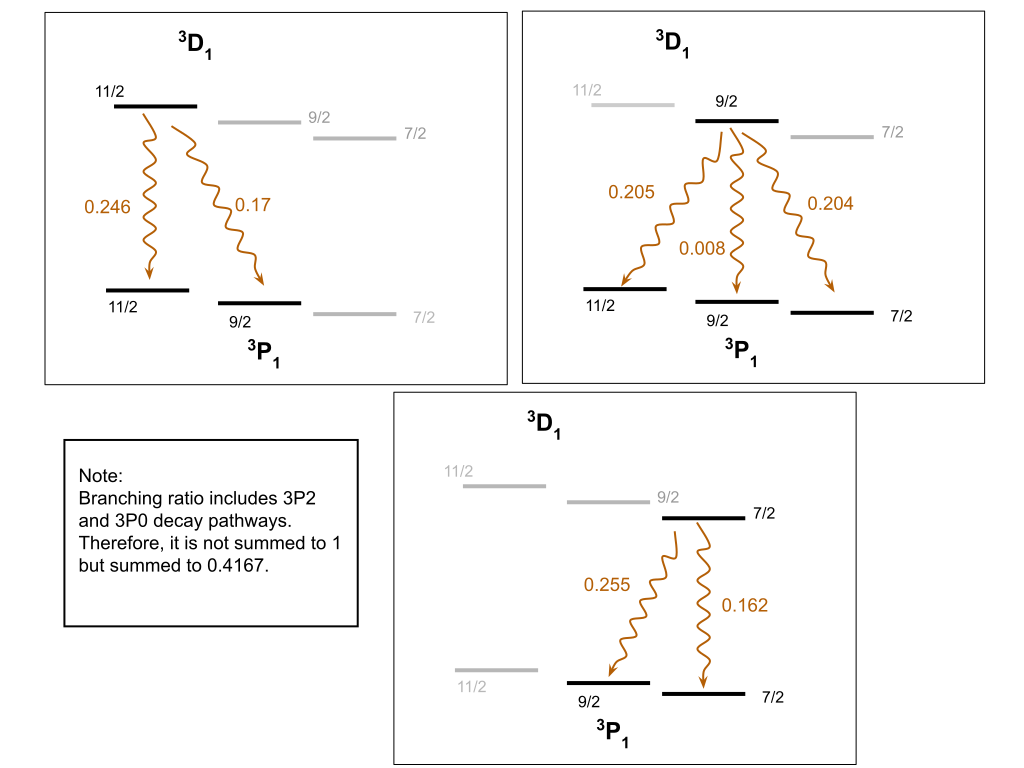
\includegraphics[width=\textwidth]{hyperfine_branching.pdf}
    \caption{Branching ratio for $\ket{^{3}D_1, F} \rightarrow \ket{^3P_1, F'}$  \label{fig:hyperfine_branching}}
\end{figure} \clearpage

\bibliographystyle{plain}
\bibliography{ref}
\end{document}